\documentclass[a4paper,12pt]{article}[abntex2]
\bibliographystyle{abntex2-alf}
\usepackage{siunitx} % Fornece suporte para a tipografia de unidades do Sistema Internacional e formatação de números
\usepackage{booktabs} % Melhora a qualidade das tabelas
\usepackage{tabularx} % Permite tabelas com larguras de colunas ajustáveis
\usepackage{graphicx} % Suporte para inclusão de imagens
\usepackage{newtxtext} % Substitui a fonte padrão pela Times Roman
\usepackage{ragged2e} % Justificação de texto melhorada
\usepackage{setspace} % Controle do espaçamento entre linhas
\usepackage[a4paper, left=3.0cm, top=3.0cm, bottom=2.0cm, rigH=2.0cm]{geometry} % Personalização das margens do documento
\usepackage{lipsum} % Geração de texto dummy 'Lorem Ipsum'
\usepackage{fancyhdr} % Customização de cabeçalhos e rodapés
\usepackage{titlesec} % Personalização dos títulos de seções
\usepackage[portuguese]{babel} % Adaptação para o português (nomes e hifenização
\usepackage{hyperref} % Suporte a hiperlinks
\usepackage{indentfirst} % Indentação do primeiro parágrafo das seções
\sisetup{
  output-decimal-marker = {,},
  inter-unit-product = \ensuremath{{}\cdot{}},
  per-mode = symbol
}
\DeclareSIUnit{\real}{R\$}
\newcommand{\real}[1]{R\$#1}
\usepackage{float} % Melhor controle sobre o posicionamento de figuras e tabelas
\usepackage{footnotehyper} % Notas de rodapé clicáveis em combinação com hyperref
\hypersetup{
    colorlinks=true,
    linkcolor=black,
    filecolor=magenta,      
    urlcolor=cyan,
    citecolor=black,        
    pdfborder={0 0 0},
}
\usepackage[normalem]{ulem} % Permite o uso de diferentes tipos de sublinhados sem alterar o \emph{}
\makeatletter
\def\@pdfborder{0 0 0} % Remove a borda dos links
\def\@pdfborderstyle{/S/U/W 1} % Estilo da borda dos links
\makeatother
\onehalfspacing
\begin{document}

\begin{titlepage}
    \centering
    \vspace*{1cm}
    \Large\textbf{INSPER – INSTITUTO DE ENSINO E PESQUISA}\\
    \Large ECONOMIA\\
    \vspace{1.5cm}
    \Large\textbf{Prova Intermediária – Primeira Parte}\\
    \textbf{Macroeconomia Internacional}\\
    \vspace{1.5cm}
    Prof. Gino Olivares\\
    Prof. Auxiliar Victor Dias \\
    \vfill
    \normalsize
    Fabrizio Antonini Ripoli, \href{mailto:fabrizioar@al.insper.edu.br}{fabrizioar@al.insper.edu.br}\\
    Hicham Munir Tayfour, \href{mailto:hichamt@al.insper.edu.br}{hichamt@al.insper.edu.br}\\
    4º Período - Economia B\\
    \vfill
    São Paulo\\
    Março/2024
\end{titlepage}

\newpage
\tableofcontents
\thispagestyle{empty} % This command removes the page number from the table of contents page
\newpage
\setcounter{page}{1} % This command sets the page number to start from this page
\justify
\onehalfspacing

\pagestyle{fancy}
\fancyhf{}
\rhead{\thepage}

\section{\textbf{Letra A}}
Construímos os gráficos da evolução histórica as curvas de Taxa Básica de Juros (TBJ), Taxa de Juros de Dois Anos (T2A) e Taxa de Câmbio Spot de Dólares Australianos por Dólares Canadenses.

A comparação entre TBJ e T2A da Austrália está na figura Figura~\ref{fig:TBJ Vs T2A (Austrália)}.

\begin{figure}[H]
    \centering
    \caption{TBJ Vs T2A (Austrália)} 
    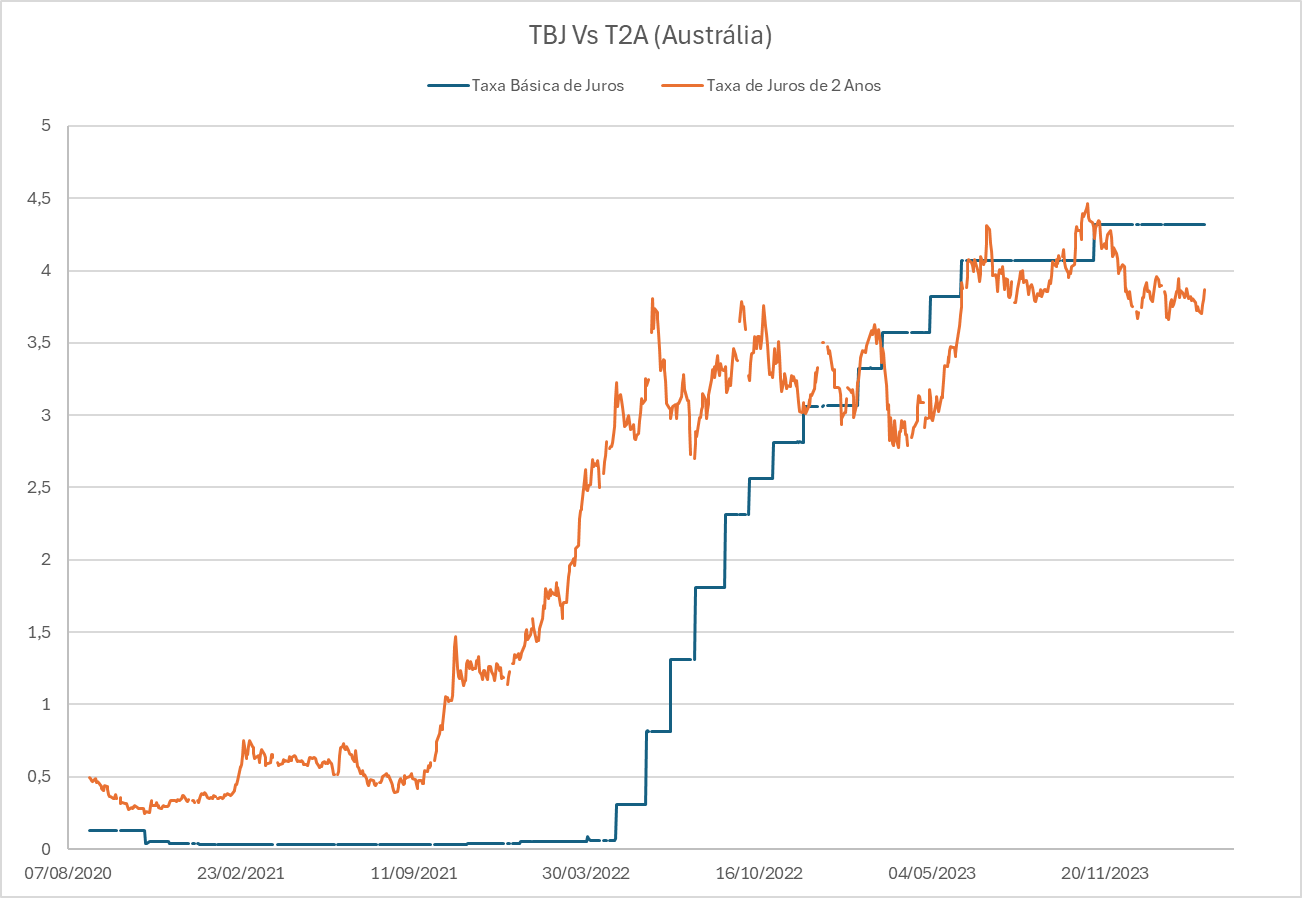
\includegraphics[width=1.0\textwidth]{TBJ Vs T2A (Austrália).png}
    \label{fig:TBJ Vs T2A (Austrália)}
    
    \footnotesize{Fonte: Elaborado pelos autores.}
    \end{figure}

A comparação entre TBJ e T2A do Canadá está na figura Figura~\ref{fig:TBJ Vs T2A (Canadá)}.

\begin{figure}[H]
    \centering
    \caption{TBJ Vs T2A (Canadá)} 
    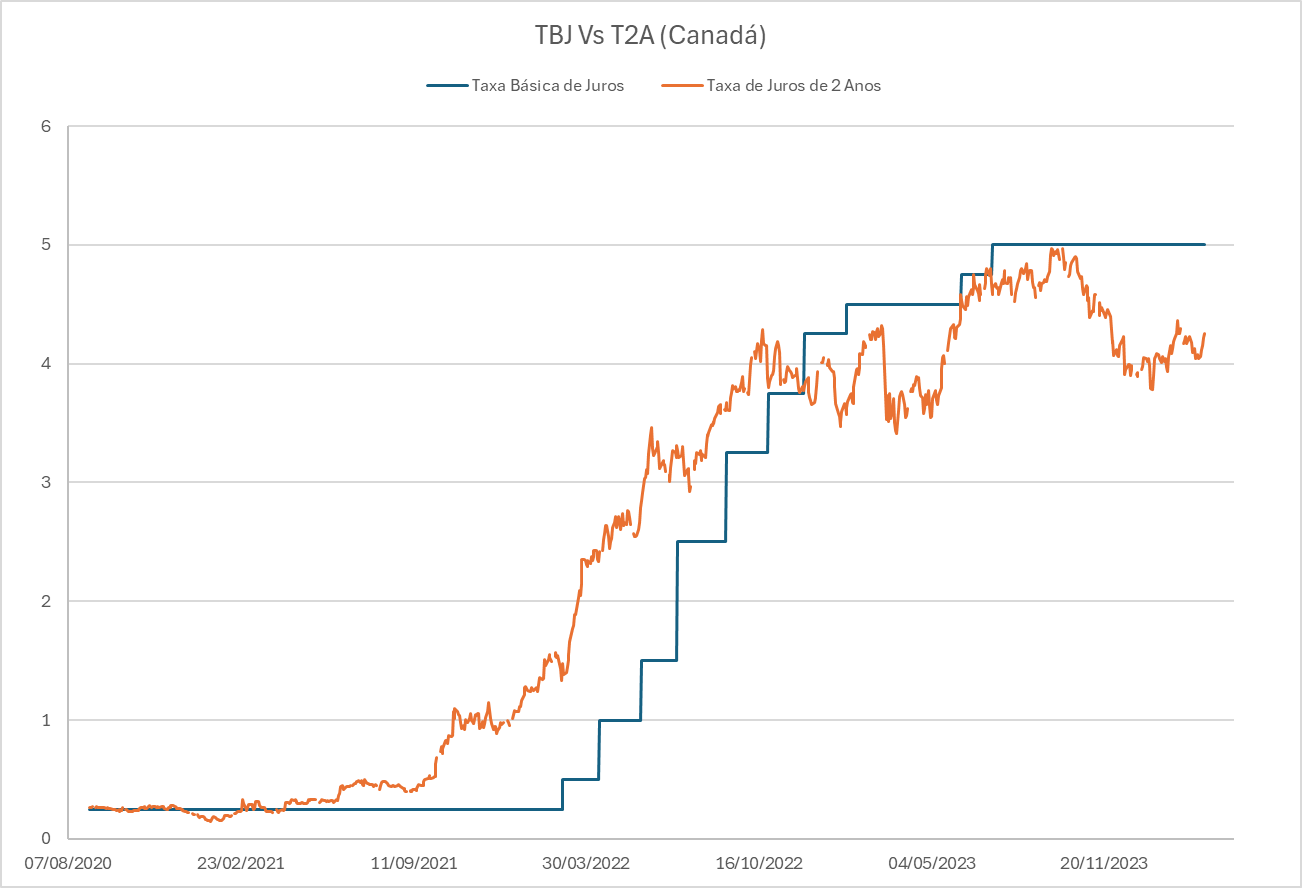
\includegraphics[width=1.0\textwidth]{TBJ Vs T2A (Canadá).png}
    \label{fig:TBJ Vs T2A (Canadá)}
    
    \footnotesize{Fonte: Elaborado pelos autores.}
    \end{figure}

Para a criação da série da taxa de câmbio dólares australianos por dólares canadenses, dividimos a taxa de câmbio de dólares australianos por dólares americanos pela taxa de câmbio de dólares canadenses por dólares americanos. Essa razão resulta na série da taxa de câmbio dólares australianos por dólares canadenses representada na Figura~\ref{fig:Câmbio Dólares Australianos por Canadenses} 

\begin{figure}[H]
    \centering
    \caption{Câmbio Dólares Australianos por Canadenses} 
    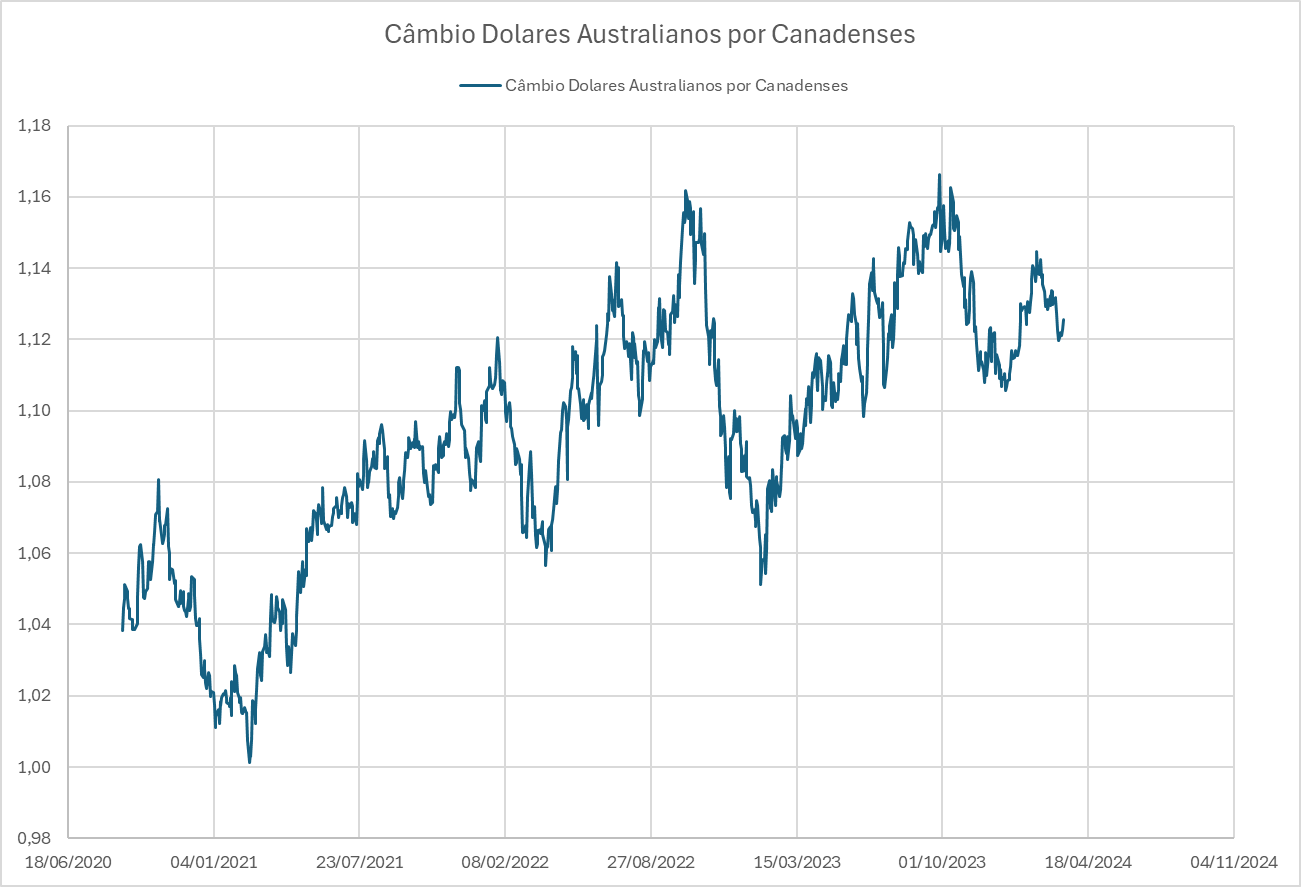
\includegraphics[width=1.0\textwidth]{Câmbio Dólares Australianos por Canadenses.png}
    \label{fig:Câmbio Dólares Australianos por Canadenses}
    
    \footnotesize{Fonte: Elaborado pelos autores.}
    \end{figure}

\section{\textbf{Letra B}}
Nessa questão, será apresentado o panorama geral dos principais acontecimentos abordados pelo E-book e considerados importantes pelo grupo. Depois disso, concluiremos com uma análise.

\subsection{\textbf{Austrália}}
\begin{itemize}
\item No início da pandemia reduziram os juros para suportar a economia e compraram títulos do governo para incentivar o crédito.
\item Em outubro não planejavam aumentar os juros por mais três anos.
\item Em novembro lançaram o GBPP (compra de títulos para incentivar os gastos em investimentos e reduzir os custos de empréstimos).
\item Em julho de 2021 houve extensão do GBPP. O projeto levou a aumento do PIB e do emprego. 
\item Em setembro de 2021 a Austrália enfrentou choque inflacionário por problemas na cadeia de suprimentos e a guerra da ucrânia com a Rússia.
\item Em dezembro de 2021 Austrália sofreu choque inflacionário por corte de fornecimento e aumento da demanda.
\item E em maio de 2022 a RBA aumentou os juros.
\end{itemize}

\subsection{\textbf{Canadá}}
\begin{itemize}
\item Em 21 e no início de 2022 o consumo de bens e políticas fiscais e monetárias estimulantes no mundo sobrecarregaram as cadeias de suprimentos levando a inflação.
\item Em janeiro de 2021 o Banco Central do Canadá antecipou o aumento da inflação pós pandemia (expectativa era que a inflação voltasse à medida que a demanda se regulasse e a oferta aumentasse).
\item Aumento dos juros, pois os choques eram considerados temporários e pela maior parte de 2021 a economia era considerada operando abaixo da sua capacidade.
\item No início de 2022 a economia parecia ter se recuperado, mas a invasão da Ucrânia aumentou preços de produtos agrícolas e petróleo.
\item Em junho a Omicron foi lançada e a economia se abriu totalmente aumentando a demanda.
\item Em 2023 o Banco Central do Canadá confirmou a tendência de desaceleração de inflação. Disseram que iriam baixar os juros se avaliassem a oferta e a demanda como equilibradas.
\item Em julho de 2023 viram evidências de excesso de demanda e aumentaram mais os juros cessando a pausa de 5 meses. 
\end{itemize}

\subsection{\textbf{Conclusão}}

Em ambas as economias, o juros foi o instrumento de política monetária durante o período analisado.

A análise parte do mesmo contexto de pós-pandemia, em que os meios de produção não conseguiram acompanhar a demanda, gerando choques nos preços.
Na Austrália, a resposta à inflação foi mais rápida mas a política monetária gerou dificuldades em controlar a oferta de moeda, já no Canadá, os juros foram alterados tardiamente assumindo que a onde de aumento de preços seria breve.

A inflação foi agravada nos dois casos com a guerra da Rússia e da Ucrânia, que restringiu a oferta.

\section{\textbf{Letra C}}
Podemos notar que a relação de câmbio de dólares australianos por canadenses, representada na figura Figura~\ref{fig:Câmbio Dólares Australianos por Canadenses}, possui um período de baixa após junho de 2020 que se encerra um pouco depois de janeiro de 2021, na qual se inicia um momento de valorização do dólar canadense em relação ao australiano, tendo poucos momentos de queda, sucedido por novas altas.

\begin{figure}[H]
    \centering
    \caption{Câmbio Dólares Australianos por Canadenses} 
    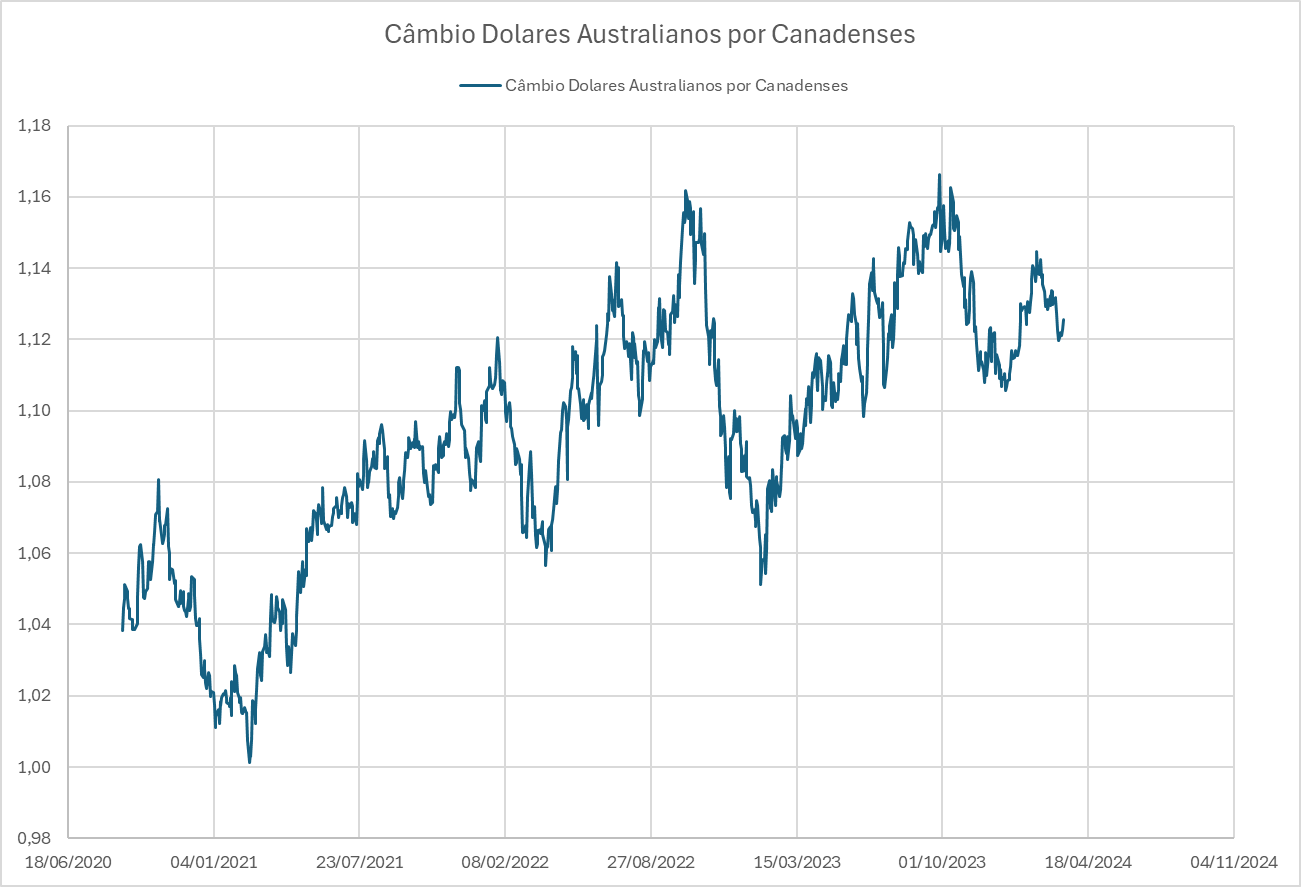
\includegraphics[width=1.0\textwidth]{Câmbio Dólares Australianos por Canadenses.png}
    \label{fig:Câmbio Dólares Australianos por Canadenses}
    
    \footnotesize{Fonte: Elaborado pelos autores.}
    \end{figure}

Um argumento econômico que pode explicar os movimentos do câmbio de dólares australianos por canadenses, seria as taxas de juros dos países. Nos momentos em que a taxa de câmbio se apreciou, pode ser devido a movimentos de aumento das taxas básicas de juros doméstica, fazendo com que a moeda tivesse sua oferta reduzida, aumentando seu valor de mercado. O raciocínio inverso também é válido.

Outro argumento econômico que pode também explicar os movimentos da taxa de câmbio, seria as taxas de juros externa. Nos momentos em que o câmbio se aprecia, pode ter sido resultado de uma redução na taxa de juros externa, fazendo com a demanda pela moeda externa diminuísse , reduzindo seu valor de mercado. O raciocínio inverso é válido aqui também.

Lembrando que tais análises levam em conta que as outras variáveis que podem alterar as taxas de câmbio estão mantidas constantes.

\section{\textbf{Letra D}}
Para a construção da série comparativa entre as taxa básicas de juros entre a Austrália e o Canadá, criamos a série diferencial que é a subtração da taxa de básica de juros da Austrália com o Canadá, onde havia valores ausentes, em qualquer uma das séries. Não consideramos esses dados para a criação do nova série, pois o resultado dela estaria impreciso , podendo gerar uma interpretação incorreta. 

A comparação entre o diferencial da taxa básica de juros e a taxa de câmbio dólares australianos por canadenses pode ser vista na Figura~\ref{fig:Comparação Diferencial TBJ e Câmbio entre os Países} 
\begin{figure}[H]
    \centering
    \caption{Comparação Diferencial TBJ e Câmbio entre os Países (AusxCan) } 
    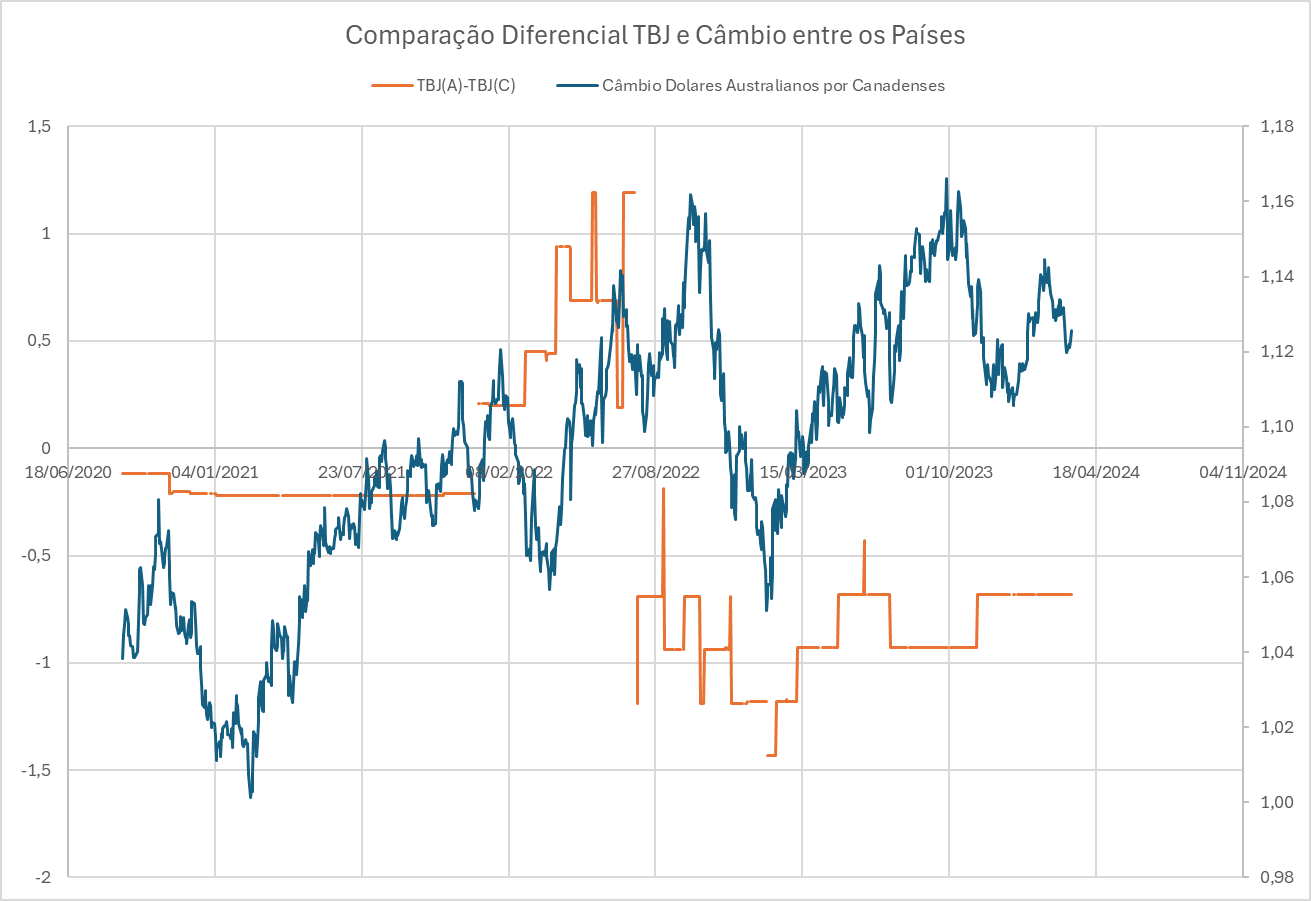
\includegraphics[width=1.0\textwidth]{Comparação Diferencial TBJ e Câmbio entre os Países.png}
    \label{fig:Comparação Diferencial TBJ e Câmbio entre os Países}
    
    \footnotesize{Fonte: Elaborado pelos autores.}
    \end{figure}

Podemos notar, visualmente que os movimentos entre o diferencial das TBJ's e a taxa de câmbio dólares australianos por canadenses possuem um alinhamento de padrão, isso pode ser evidenciado pelo calculo da correlação que resultou em um valor de -0,3045, um valor considerado de correlação baixo, mas há correlação entre a TBJ e a taxa de câmbio.

\section{\textbf{Letra E}}
Para a construção da série comparativa entre as taxa básicas de juros entre a Austrália e o Canadá, criamos a série diferencial que é a subtração da taxa de básica de juros de dois anos da Austrália com o Canadá, onde havia valores ausentes, em qualquer uma das séries. Não consideramos esses dados para a criação do nova série, pois o resultado dela estaria impreciso , podendo gerar uma interpretação incorreta. 

A comparação entre o diferencial da taxa básica de juros de dois anos e a taxa de câmbio dólares australianos por canadenses pode ser vista na  Figura~\ref{fig:Comparação Diferencial T2A e Câmbio entre os Países (AusxCan)}.
\begin{figure}[H]
    \centering
    \caption{Comparação Diferencial T2A e Câmbio entre os Países (AusxCan)} 
    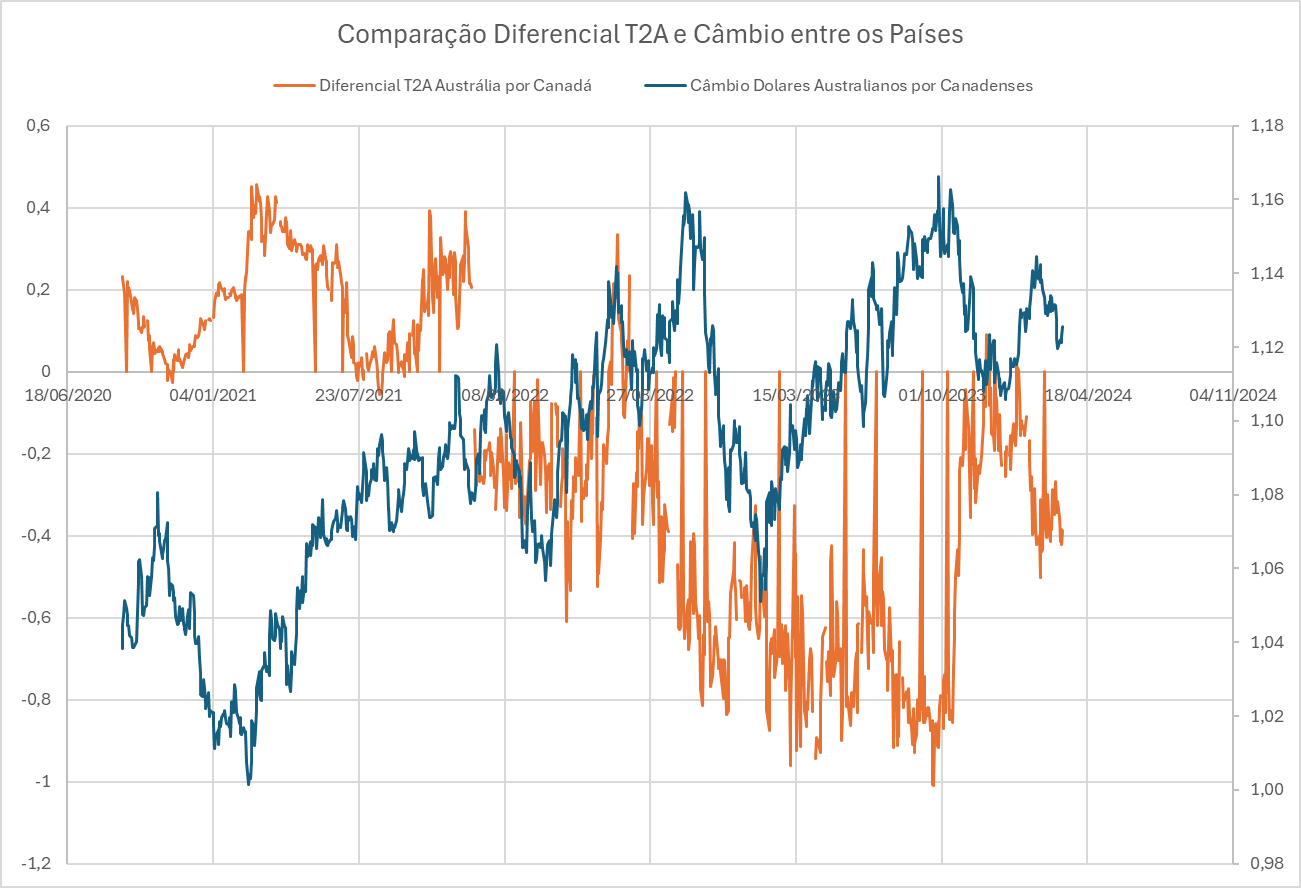
\includegraphics[width=1.0\textwidth]{Comparação Diferencial T2A e Câmbio entre os Países (AusxCan).png}
    \label{fig:Comparação Diferencial T2A e Câmbio entre os Países (AusxCan)}
    
    \footnotesize{Fonte: Elaborado pelos autores.}
    \end{figure}

Podemos notar, visualmente que os movimentos entre o diferencial das T2A's e a taxa de câmbio dólares australianos por canadenses possuem um alinhamento de padrão, isso pode ser evidenciado pelo calculo da correlação que resultou em um valor de -0,6642, um valor considerado de correlação moderado-alto, mas há correlação entre a T2A's e a taxa de câmbio.


\section{\textbf{Letra F}}

Partindo da relação de Fisher(\textbf{1}) vista em aula, relacionamos a taxa de depreciação esperada do câmbio como sendo igual à diferença das taxas de juros. Isso é dado apenas em um contexto de longo prazo teórico. A intuição é que se a taxa de juros A for maior que a C, haverá aumento da demanda por moeda de A, valorizando ela em relação à taxa de juros C.

R_{A} -  R_{C} = \frac{E_{A|C}^{e} - E_{A|C}}{E_{A|C}} (\textbf{3})

\pi_{A}^{e} - \pi_{C}^{e} = \frac{E_{A|C}^{e} - E_{A|C}}{E_{A|C}}

R_{A} -  R_{C} = \pi_{A}^{e} - \pi_{C}^{e}  (\textbf{1})

R_{A} -  \pi_{A}^{e} = R_{C} - \pi_{C}^{e} (\textbf{2})

A série que se relaciona melhor com variação da taxa de câmbio é a série do diferencial da T2A de cada país, pois é no longo prazo que todas as variáveis se ajustam, inclusive os preços.

O aumento dos preços é a inflação, e para conter a inflação o aumento da taxa de juros se faz necessário para manter o retorno real, que é diferença da taxa de juros pela inflação esperada, representada pela equação (\textbf{2}), onde a diferença de inflação esperada é dada pelo taxa de depreciação esperada (\textbf{3}).

 Caso a T2A suba, é esperado que o valor do câmbio esperado também aumente, fazendo com que a taxa de depreciação esperada siga na mesma direção no longo prazo.

Retomando o que foi dito no início, levando em consideração o diferencial da T2A entre os países, caso ele seja positivo, é esperado que o valor da moeda australiana se aprecie frente a canadense, fazendo com que o câmbio se aprecie. Caso ele seja negativo, esperamos que o câmbio se deprecie, devido a valorização do moeda canadense.


\section{\textbf{Letra G}}
Em relação a esse exercício, aprendemos a organizar dados para sua manipulação, excluir dados faltantes para não afetar a análise final. Além disso, aprendemos a organizar os gráficos de maneira a ajudar a visualizar dos dados. 

A extração das informações, presentes no \textit{e-book} sobre as políticas monetárias e suas consequências na inflação, a dinamicidade da economia e erros de cada politica. 

A realização em dupla deste trabalho ajudou na visualização de mais de uma causa para o efeito de certas relações econômicas. Além disso, a possibilidade de diálogo entre outros grupos propiciou a indagações que resultaram em novas conclusões a respeito das variáveis macroeconômicas analisadas.

Em suma, aprendemos que a análise macroeconômica requer mais de uma visão sistêmica dos processos que ocorrem no mundo, a necessidade de avaliar se fatos externos vão ou não afetar as variáveis analisadas, a necessidade de se ter um embasamento teórico para análise. Apesar do mundo real não se comportar da mesma forma que o modelo teórico afirma, ele é a base para entender como as variáveis macroeconômicas se relacionam.

\newpage
\begin{thebibliography}{9}
\section*{Bibliografia Consultada}
\bibitem{english2024monetary} 
ENGLISH, Bill; FORBES, Kristin; UBIDE, Angel (Eds.). 
\textit{Monetary Policy Responses to the Post-Pandemic Inflation}. 
London, UK: CEPR Press, 2024. E-book. ISBN 978-1-912179-82-4.  
Acesso em: 21 mar. 2024.

\bibitem{fry-mckibbin2024australia} 
FRY-MCKIBBIN, Renée A.; WILKINS, Carolyn A. 
\textit{Central Bank Responses to the Post-COVID Period of High Inflation: The Case of Australia}. In: ENGLISH, Bill; FORBES, Kristin; UBIDE, Angel (Eds.). 
\textit{Monetary Policy Responses to the Post-Pandemic Inflation}. 
London, UK: CEPR Press, 2024, p. 33-50. E-book. ISBN 978-1-912179-82-4.

\bibitem{macklem2024canada} 
MACKLEM, Tiff. 
\textit{The Bank of Canada’s Response to Post-COVID Inflation and Some Lessons Learned}. In: ENGLISH, Bill; FORBES, Kristin; UBIDE, Angel (Eds.). 
\textit{Monetary Policy Responses to the Post-Pandemic Inflation}. 
London, UK: CEPR Press, 2024, p. 51-64. E-book. ISBN 978-1-912179-82-4.
\end{thebibliography}

\end{document}
